\documentclass[1p]{elsarticle_modified}
%\bibliographystyle{elsarticle-num}

%\usepackage[colorlinks]{hyperref}
%\usepackage{abbrmath_seonhwa} %\Abb, \Ascr, \Acal ,\Abf, \Afrak
\usepackage{amsfonts}
\usepackage{amssymb}
\usepackage{amsmath}
\usepackage{amsthm}
\usepackage{scalefnt}
\usepackage{amsbsy}
\usepackage{kotex}
\usepackage{caption}
\usepackage{subfig}
\usepackage{color}
\usepackage{graphicx}
\usepackage{xcolor} %% white, black, red, green, blue, cyan, magenta, yellow
\usepackage{float}
\usepackage{setspace}
\usepackage{hyperref}

\usepackage{tikz}
\usetikzlibrary{arrows}

\usepackage{multirow}
\usepackage{array} % fixed length table
\usepackage{hhline}

%%%%%%%%%%%%%%%%%%%%%
\makeatletter
\renewcommand*\env@matrix[1][\arraystretch]{%
	\edef\arraystretch{#1}%
	\hskip -\arraycolsep
	\let\@ifnextchar\new@ifnextchar
	\array{*\c@MaxMatrixCols c}}
\makeatother %https://tex.stackexchange.com/questions/14071/how-can-i-increase-the-line-spacing-in-a-matrix
%%%%%%%%%%%%%%%

\usepackage[normalem]{ulem}

\newcommand{\msout}[1]{\ifmmode\text{\sout{\ensuremath{#1}}}\else\sout{#1}\fi}
%SOURCE: \msout is \stkout macro in https://tex.stackexchange.com/questions/20609/strikeout-in-math-mode

\newcommand{\cancel}[1]{
	\ifmmode
	{\color{red}\msout{#1}}
	\else
	{\color{red}\sout{#1}}
	\fi
}

\newcommand{\add}[1]{
	{\color{blue}\uwave{#1}}
}

\newcommand{\replace}[2]{
	\ifmmode
	{\color{red}\msout{#1}}{\color{blue}\uwave{#2}}
	\else
	{\color{red}\sout{#1}}{\color{blue}\uwave{#2}}
	\fi
}

\newcommand{\Sol}{\mathcal{S}} %segment
\newcommand{\D}{D} %diagram
\newcommand{\A}{\mathcal{A}} %arc


%%%%%%%%%%%%%%%%%%%%%%%%%%%%%5 test

\def\sl{\operatorname{\textup{SL}}(2,\Cbb)}
\def\psl{\operatorname{\textup{PSL}}(2,\Cbb)}
\def\quan{\mkern 1mu \triangleright \mkern 1mu}

\theoremstyle{definition}
\newtheorem{thm}{Theorem}[section]
\newtheorem{prop}[thm]{Proposition}
\newtheorem{lem}[thm]{Lemma}
\newtheorem{ques}[thm]{Question}
\newtheorem{cor}[thm]{Corollary}
\newtheorem{defn}[thm]{Definition}
\newtheorem{exam}[thm]{Example}
\newtheorem{rmk}[thm]{Remark}
\newtheorem{alg}[thm]{Algorithm}

\newcommand{\I}{\sqrt{-1}}
\begin{document}

%\begin{frontmatter}
%
%\title{Boundary parabolic representations of knots up to 8 crossings}
%
%%% Group authors per affiliation:
%\author{Yunhi Cho} 
%\address{Department of Mathematics, University of Seoul, Seoul, Korea}
%\ead{yhcho@uos.ac.kr}
%
%
%\author{Seonhwa Kim} %\fnref{s_kim}}
%\address{Center for Geometry and Physics, Institute for Basic Science, Pohang, 37673, Korea}
%\ead{ryeona17@ibs.re.kr}
%
%\author{Hyuk Kim}
%\address{Department of Mathematical Sciences, Seoul National University, Seoul 08826, Korea}
%\ead{hyukkim@snu.ac.kr}
%
%\author{Seokbeom Yoon}
%\address{Department of Mathematical Sciences, Seoul National University, Seoul, 08826,  Korea}
%\ead{sbyoon15@snu.ac.kr}
%
%\begin{abstract}
%We find all boundary parabolic representation of knots up to 8 crossings.
%
%\end{abstract}
%\begin{keyword}
%    \MSC[2010] 57M25 
%\end{keyword}
%
%\end{frontmatter}

%\linenumbers
%\tableofcontents
%
\newcommand\colored[1]{\textcolor{white}{\rule[-0.35ex]{0.8em}{1.4ex}}\kern-0.8em\color{red} #1}%
%\newcommand\colored[1]{\textcolor{white}{ #1}\kern-2.17ex	\textcolor{white}{ #1}\kern-1.81ex	\textcolor{white}{ #1}\kern-2.15ex\color{red}#1	}

{\Large $\underline{12a_{1194}~(K12a_{1194})}$}

\setlength{\tabcolsep}{10pt}
\renewcommand{\arraystretch}{1.6}
\vspace{1cm}\begin{tabular}{m{100pt}>{\centering\arraybackslash}m{274pt}}
\multirow{5}{120pt}{
	\centering
	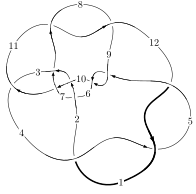
\includegraphics[width=112pt]{../../../GIT/diagram.site/Diagrams/png/1995_12a_1194.png}\\
\ \ \ A knot diagram\footnotemark}&
\allowdisplaybreaks
\textbf{Linearized knot diagam} \\
\cline{2-2}
 &
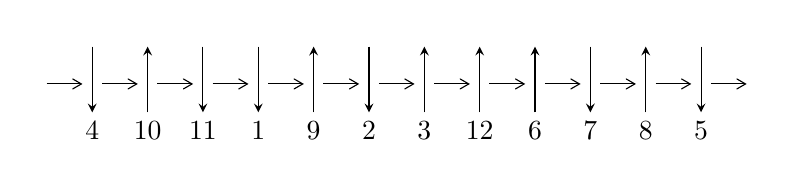
\begin{tikzpicture}[x=20pt, y=17pt]
	% nodes
	\node (C0) at (0, 0) {};
	\node (C1) at (1, 0) {};
	\node (C1U) at (1, +1) {};
	\node (C1D) at (1, -1) {4};

	\node (C2) at (2, 0) {};
	\node (C2U) at (2, +1) {};
	\node (C2D) at (2, -1) {10};

	\node (C3) at (3, 0) {};
	\node (C3U) at (3, +1) {};
	\node (C3D) at (3, -1) {11};

	\node (C4) at (4, 0) {};
	\node (C4U) at (4, +1) {};
	\node (C4D) at (4, -1) {1};

	\node (C5) at (5, 0) {};
	\node (C5U) at (5, +1) {};
	\node (C5D) at (5, -1) {9};

	\node (C6) at (6, 0) {};
	\node (C6U) at (6, +1) {};
	\node (C6D) at (6, -1) {2};

	\node (C7) at (7, 0) {};
	\node (C7U) at (7, +1) {};
	\node (C7D) at (7, -1) {3};

	\node (C8) at (8, 0) {};
	\node (C8U) at (8, +1) {};
	\node (C8D) at (8, -1) {12};

	\node (C9) at (9, 0) {};
	\node (C9U) at (9, +1) {};
	\node (C9D) at (9, -1) {6};

	\node (C10) at (10, 0) {};
	\node (C10U) at (10, +1) {};
	\node (C10D) at (10, -1) {7};

	\node (C11) at (11, 0) {};
	\node (C11U) at (11, +1) {};
	\node (C11D) at (11, -1) {8};

	\node (C12) at (12, 0) {};
	\node (C12U) at (12, +1) {};
	\node (C12D) at (12, -1) {5};
	\node (C13) at (13, 0) {};

	% arrows
	\draw[->,>={angle 60}]
	(C0) edge (C1) (C1) edge (C2) (C2) edge (C3) (C3) edge (C4) (C4) edge (C5) (C5) edge (C6) (C6) edge (C7) (C7) edge (C8) (C8) edge (C9) (C9) edge (C10) (C10) edge (C11) (C11) edge (C12) (C12) edge (C13) ;	\draw[->,>=stealth]
	(C1U) edge (C1D) (C2D) edge (C2U) (C3U) edge (C3D) (C4U) edge (C4D) (C5D) edge (C5U) (C6U) edge (C6D) (C7D) edge (C7U) (C8D) edge (C8U) (C9D) edge (C9U) (C10U) edge (C10D) (C11D) edge (C11U) (C12U) edge (C12D) ;
	\end{tikzpicture} \\
\hhline{~~} \\& 
\textbf{Solving Sequence} \\ \cline{2-2} 
 &
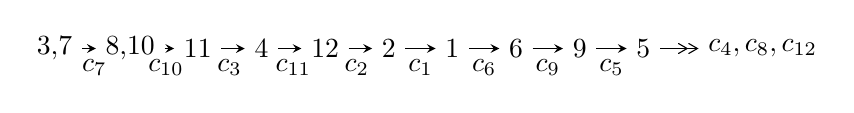
\begin{tikzpicture}[x=23pt, y=7pt]
	% node
	\node (A0) at (-1/8, 0) {3,7};
	\node (A1) at (17/16, 0) {8,10};
	\node (A2) at (17/8, 0) {11};
	\node (A3) at (25/8, 0) {4};
	\node (A4) at (33/8, 0) {12};
	\node (A5) at (41/8, 0) {2};
	\node (A6) at (49/8, 0) {1};
	\node (A7) at (57/8, 0) {6};
	\node (A8) at (65/8, 0) {9};
	\node (A9) at (73/8, 0) {5};
	\node (C1) at (1/2, -1) {$c_{7}$};
	\node (C2) at (13/8, -1) {$c_{10}$};
	\node (C3) at (21/8, -1) {$c_{3}$};
	\node (C4) at (29/8, -1) {$c_{11}$};
	\node (C5) at (37/8, -1) {$c_{2}$};
	\node (C6) at (45/8, -1) {$c_{1}$};
	\node (C7) at (53/8, -1) {$c_{6}$};
	\node (C8) at (61/8, -1) {$c_{9}$};
	\node (C9) at (69/8, -1) {$c_{5}$};
	\node (A10) at (11, 0) {$c_{4},c_{8},c_{12}$};

	% edge
	\draw[->,>=stealth]	
	(A0) edge (A1) (A1) edge (A2) (A2) edge (A3) (A3) edge (A4) (A4) edge (A5) (A5) edge (A6) (A6) edge (A7) (A7) edge (A8) (A8) edge (A9) ;
	\draw[->>,>={angle 60}]	
	(A9) edge (A10);
\end{tikzpicture} \\ 

\end{tabular} \\

\footnotetext{
The image of knot diagram is generated by the software ``\textbf{Draw programme}" developed by Andrew Bartholomew(\url{http://www.layer8.co.uk/maths/draw/index.htm\#Running-draw}), where we modified some parts for our purpose(\url{https://github.com/CATsTAILs/LinksPainter}).
}\phantom \\ \newline 
\centering \textbf{Ideals for irreducible components\footnotemark of $X_{\text{par}}$} 
 
\begin{align*}
I^u_{1}&=\langle 
9.79780\times10^{46} u^{37}+3.35501\times10^{46} u^{36}+\cdots+1.92279\times10^{47} b-2.18034\times10^{47},\;a-1,\\
\phantom{I^u_{1}}&\phantom{= \langle  }u^{38}+u^{37}+\cdots+19 u^2-1\rangle \\
I^u_{2}&=\langle 
1.82885\times10^{255} u^{71}-9.62892\times10^{254} u^{70}+\cdots+6.92537\times10^{255} b+6.25833\times10^{257},\\
\phantom{I^u_{2}}&\phantom{= \langle  }1.88860\times10^{255} u^{71}-1.18895\times10^{255} u^{70}+\cdots+6.92537\times10^{255} a+4.84199\times10^{257},\\
\phantom{I^u_{2}}&\phantom{= \langle  }u^{72}+u^{70}+\cdots+600 u+192\rangle \\
I^u_{3}&=\langle 
- u^{15}- u^{14}+u^{11}-2 u^{10}-6 u^9-5 u^8+9 u^7-13 u^6-5 u^5+30 u^4+u^3-25 u^2+b+8,\;a+1,\\
\phantom{I^u_{3}}&\phantom{= \langle  }u^{17}- u^{14}+u^{12}+6 u^{11}-2 u^{10}-7 u^9+13 u^8-6 u^7-24 u^6+12 u^5+19 u^4-6 u^3-7 u^2+u+1\rangle \\
I^u_{4}&=\langle 
3 b+u-2,\;a- u-1,\;u^2- u+1\rangle \\
I^u_{5}&=\langle 
6 b- u-3,\;6 a- u-3,\;u^2+3\rangle \\
I^u_{6}&=\langle 
b+1,\;a+1,\;u^2- u+1\rangle \\
\\
\end{align*}
\raggedright * 6 irreducible components of $\dim_{\mathbb{C}}=0$, with total 133 representations.\\
\footnotetext{All coefficients of polynomials are rational numbers. But the coefficients are sometimes approximated in decimal forms when there is not enough margin.}
\newpage
\renewcommand{\arraystretch}{1}
\centering \section*{I. $I^u_{1}= \langle 9.80\times10^{46} u^{37}+3.36\times10^{46} u^{36}+\cdots+1.92\times10^{47} b-2.18\times10^{47},\;a-1,\;u^{38}+u^{37}+\cdots+19 u^2-1 \rangle$}
\flushleft \textbf{(i) Arc colorings}\\
\begin{tabular}{m{7pt} m{180pt} m{7pt} m{180pt} }
\flushright $a_{3}=$&$\begin{pmatrix}0\\u\end{pmatrix}$ \\
\flushright $a_{7}=$&$\begin{pmatrix}1\\0\end{pmatrix}$ \\
\flushright $a_{8}=$&$\begin{pmatrix}1\\- u^2\end{pmatrix}$ \\
\flushright $a_{10}=$&$\begin{pmatrix}1\\-0.509562 u^{37}-0.174487 u^{36}+\cdots-3.84868 u+1.13395\end{pmatrix}$ \\
\flushright $a_{11}=$&$\begin{pmatrix}0.509562 u^{37}+0.174487 u^{36}+\cdots+3.84868 u-0.133946\\-0.509562 u^{37}-0.174487 u^{36}+\cdots-3.84868 u+1.13395\end{pmatrix}$ \\
\flushright $a_{4}=$&$\begin{pmatrix}1.24784 u^{37}+1.13746 u^{36}+\cdots+6.22030 u-2.73265\\-0.912766 u^{37}-0.757139 u^{36}+\cdots-5.08636 u+2.22309\end{pmatrix}$ \\
\flushright $a_{12}=$&$\begin{pmatrix}-0.0452476 u^{37}-0.116918 u^{36}+\cdots+0.509562 u+0.664925\\-0.448231 u^{37}-0.142720 u^{36}+\cdots-3.29387 u+0.870541\end{pmatrix}$ \\
\flushright $a_{2}=$&$\begin{pmatrix}- u\\-0.335075 u^{37}-0.380323 u^{36}+\cdots-0.133946 u+0.509562\end{pmatrix}$ \\
\flushright $a_{1}=$&$\begin{pmatrix}-1.54245 u^{37}-1.84686 u^{36}+\cdots-19.6552 u+3.53329\\0.666260 u^{37}+0.909070 u^{36}+\cdots+13.3755 u-2.01544\end{pmatrix}$ \\
\flushright $a_{6}=$&$\begin{pmatrix}-0.0452476 u^{37}-0.116918 u^{36}+\cdots+0.509562 u+0.664925\\-0.110380 u^{37}+0.0315993 u^{36}+\cdots-2.73265 u+1.24784\end{pmatrix}$ \\
\flushright $a_{9}=$&$\begin{pmatrix}0.915215 u^{37}+0.651574 u^{36}+\cdots+5.45183 u-0.569657\\-1.33092 u^{37}-0.844964 u^{36}+\cdots-10.0710 u+3.53250\end{pmatrix}$ \\
\flushright $a_{5}=$&$\begin{pmatrix}-2.03274 u^{37}-1.11723 u^{36}+\cdots-15.2736 u+6.20954\\2.05290 u^{37}+1.33796 u^{36}+\cdots+17.7773 u-6.02161\end{pmatrix}$\\&\end{tabular}
\flushleft \textbf{(ii) Obstruction class $= -1$}\\~\\
\flushleft \textbf{(iii) Cusp Shapes $= -0.739502 u^{37}-0.948748 u^{36}+\cdots-10.0381 u+6.25697$}\\~\\
\newpage\renewcommand{\arraystretch}{1}
\flushleft \textbf{(iv) u-Polynomials at the component}\newline \\
\begin{tabular}{m{50pt}|m{274pt}}
Crossings & \hspace{64pt}u-Polynomials at each crossing \\
\hline $$\begin{aligned}c_{1},c_{4},c_{12}\end{aligned}$$&$\begin{aligned}
&u^{38}-10 u^{37}+\cdots+208 u-16
\end{aligned}$\\
\hline $$\begin{aligned}c_{2},c_{7}\end{aligned}$$&$\begin{aligned}
&u^{38}+u^{37}+\cdots+19 u^2-1
\end{aligned}$\\
\hline $$\begin{aligned}c_{3},c_{6}\end{aligned}$$&$\begin{aligned}
&u^{38}+u^{37}+\cdots-8 u-4
\end{aligned}$\\
\hline $$\begin{aligned}c_{5},c_{8},c_{9}\\c_{11}\end{aligned}$$&$\begin{aligned}
&u^{38}-22 u^{36}+\cdots+12 u+1
\end{aligned}$\\
\hline $$\begin{aligned}c_{10}\end{aligned}$$&$\begin{aligned}
&u^{38}+18 u^{37}+\cdots-62 u-4
\end{aligned}$\\
\hline
\end{tabular}\\~\\
\newpage\renewcommand{\arraystretch}{1}
\flushleft \textbf{(v) Riley Polynomials at the component}\newline \\
\begin{tabular}{m{50pt}|m{274pt}}
Crossings & \hspace{64pt}Riley Polynomials at each crossing \\
\hline $$\begin{aligned}c_{1},c_{4},c_{12}\end{aligned}$$&$\begin{aligned}
&y^{38}+38 y^{37}+\cdots+2016 y+256
\end{aligned}$\\
\hline $$\begin{aligned}c_{2},c_{7}\end{aligned}$$&$\begin{aligned}
&y^{38}-19 y^{37}+\cdots-38 y+1
\end{aligned}$\\
\hline $$\begin{aligned}c_{3},c_{6}\end{aligned}$$&$\begin{aligned}
&y^{38}+7 y^{37}+\cdots+264 y+16
\end{aligned}$\\
\hline $$\begin{aligned}c_{5},c_{8},c_{9}\\c_{11}\end{aligned}$$&$\begin{aligned}
&y^{38}-44 y^{37}+\cdots-50 y+1
\end{aligned}$\\
\hline $$\begin{aligned}c_{10}\end{aligned}$$&$\begin{aligned}
&y^{38}-4 y^{37}+\cdots-716 y+16
\end{aligned}$\\
\hline
\end{tabular}\\~\\
\newpage\flushleft \textbf{(vi) Complex Volumes and Cusp Shapes}
$$\begin{array}{c|c|c}  
\text{Solutions to }I^u_{1}& \I (\text{vol} + \sqrt{-1}CS) & \text{Cusp shape}\\
 \hline 
\begin{aligned}
u &= \phantom{-}0.479520 + 0.882461 I \\
a &= \phantom{-}1.00000\phantom{ +0.000000I} \\
b &= \phantom{-}0.751362 - 0.367985 I\end{aligned}
 & -0.19527 + 1.57472 I & -3.21629 - 2.23777 I \\ \hline\begin{aligned}
u &= \phantom{-}0.479520 - 0.882461 I \\
a &= \phantom{-}1.00000\phantom{ +0.000000I} \\
b &= \phantom{-}0.751362 + 0.367985 I\end{aligned}
 & -0.19527 - 1.57472 I & -3.21629 + 2.23777 I \\ \hline\begin{aligned}
u &= \phantom{-}0.644139 + 0.745875 I \\
a &= \phantom{-}1.00000\phantom{ +0.000000I} \\
b &= \phantom{-}0.822899 - 0.634508 I\end{aligned}
 & -0.13192 + 1.60989 I & -0.75540 - 1.36355 I \\ \hline\begin{aligned}
u &= \phantom{-}0.644139 - 0.745875 I \\
a &= \phantom{-}1.00000\phantom{ +0.000000I} \\
b &= \phantom{-}0.822899 + 0.634508 I\end{aligned}
 & -0.13192 - 1.60989 I & -0.75540 + 1.36355 I \\ \hline\begin{aligned}
u &= -0.937133 + 0.239327 I \\
a &= \phantom{-}1.00000\phantom{ +0.000000I} \\
b &= \phantom{-}0.76066 - 1.21673 I\end{aligned}
 & \phantom{-}9.11838 - 5.83428 I & \phantom{-}8.14618 + 5.74561 I \\ \hline\begin{aligned}
u &= -0.937133 - 0.239327 I \\
a &= \phantom{-}1.00000\phantom{ +0.000000I} \\
b &= \phantom{-}0.76066 + 1.21673 I\end{aligned}
 & \phantom{-}9.11838 + 5.83428 I & \phantom{-}8.14618 - 5.74561 I \\ \hline\begin{aligned}
u &= \phantom{-}0.852502 + 0.278386 I \\
a &= \phantom{-}1.00000\phantom{ +0.000000I} \\
b &= \phantom{-}0.95818 + 1.45928 I\end{aligned}
 & \phantom{-}16.3227 + 9.5388 I & \phantom{-}10.67449 - 6.03102 I \\ \hline\begin{aligned}
u &= \phantom{-}0.852502 - 0.278386 I \\
a &= \phantom{-}1.00000\phantom{ +0.000000I} \\
b &= \phantom{-}0.95818 - 1.45928 I\end{aligned}
 & \phantom{-}16.3227 - 9.5388 I & \phantom{-}10.67449 + 6.03102 I \\ \hline\begin{aligned}
u &= -0.871208 + 0.681798 I \\
a &= \phantom{-}1.00000\phantom{ +0.000000I} \\
b &= \phantom{-}1.16064 + 0.91404 I\end{aligned}
 & -1.77981 - 4.59053 I & -3.12624 + 6.99491 I \\ \hline\begin{aligned}
u &= -0.871208 - 0.681798 I \\
a &= \phantom{-}1.00000\phantom{ +0.000000I} \\
b &= \phantom{-}1.16064 - 0.91404 I\end{aligned}
 & -1.77981 + 4.59053 I & -3.12624 - 6.99491 I\\
 \hline 
 \end{array}$$\newpage$$\begin{array}{c|c|c}  
\text{Solutions to }I^u_{1}& \I (\text{vol} + \sqrt{-1}CS) & \text{Cusp shape}\\
 \hline 
\begin{aligned}
u &= \phantom{-}1.098320 + 0.234964 I \\
a &= \phantom{-}1.00000\phantom{ +0.000000I} \\
b &= \phantom{-}0.682932 + 0.779615 I\end{aligned}
 & \phantom{-}8.59426 + 0.71431 I & \phantom{-}7.79538 + 0.07256 I \\ \hline\begin{aligned}
u &= \phantom{-}1.098320 - 0.234964 I \\
a &= \phantom{-}1.00000\phantom{ +0.000000I} \\
b &= \phantom{-}0.682932 - 0.779615 I\end{aligned}
 & \phantom{-}8.59426 - 0.71431 I & \phantom{-}7.79538 - 0.07256 I \\ \hline\begin{aligned}
u &= \phantom{-}0.957238 + 0.605348 I \\
a &= \phantom{-}1.00000\phantom{ +0.000000I} \\
b &= \phantom{-}1.27321 - 1.10751 I\end{aligned}
 & \phantom{-}3.03840 + 7.55076 I & \phantom{-}2.62397 - 7.06584 I \\ \hline\begin{aligned}
u &= \phantom{-}0.957238 - 0.605348 I \\
a &= \phantom{-}1.00000\phantom{ +0.000000I} \\
b &= \phantom{-}1.27321 + 1.10751 I\end{aligned}
 & \phantom{-}3.03840 - 7.55076 I & \phantom{-}2.62397 + 7.06584 I \\ \hline\begin{aligned}
u &= -0.666023 + 0.378508 I \\
a &= \phantom{-}1.00000\phantom{ +0.000000I} \\
b &= \phantom{-}0.385427 + 1.322160 I\end{aligned}
 & \phantom{-}5.43833 - 1.25341 I & \phantom{-}5.66766 + 5.57255 I \\ \hline\begin{aligned}
u &= -0.666023 - 0.378508 I \\
a &= \phantom{-}1.00000\phantom{ +0.000000I} \\
b &= \phantom{-}0.385427 - 1.322160 I\end{aligned}
 & \phantom{-}5.43833 + 1.25341 I & \phantom{-}5.66766 - 5.57255 I \\ \hline\begin{aligned}
u &= \phantom{-}0.753740 + 0.136199 I \\
a &= \phantom{-}1.00000\phantom{ +0.000000I} \\
b &= -0.541177 - 0.389347 I\end{aligned}
 & \phantom{-}2.42366 - 3.68294 I & -1.25459 - 4.84612 I \\ \hline\begin{aligned}
u &= \phantom{-}0.753740 - 0.136199 I \\
a &= \phantom{-}1.00000\phantom{ +0.000000I} \\
b &= -0.541177 + 0.389347 I\end{aligned}
 & \phantom{-}2.42366 + 3.68294 I & -1.25459 + 4.84612 I \\ \hline\begin{aligned}
u &= -1.241290 + 0.060112 I \\
a &= \phantom{-}1.00000\phantom{ +0.000000I} \\
b &= -0.159015 + 0.380020 I\end{aligned}
 & \phantom{-}14.1852 - 1.9882 I & \phantom{-}9.99909 + 0.39309 I \\ \hline\begin{aligned}
u &= -1.241290 - 0.060112 I \\
a &= \phantom{-}1.00000\phantom{ +0.000000I} \\
b &= -0.159015 - 0.380020 I\end{aligned}
 & \phantom{-}14.1852 + 1.9882 I & \phantom{-}9.99909 - 0.39309 I\\
 \hline 
 \end{array}$$\newpage$$\begin{array}{c|c|c}  
\text{Solutions to }I^u_{1}& \I (\text{vol} + \sqrt{-1}CS) & \text{Cusp shape}\\
 \hline 
\begin{aligned}
u &= \phantom{-}1.27422\phantom{ +0.000000I} \\
a &= \phantom{-}1.00000\phantom{ +0.000000I} \\
b &= \phantom{-}0.155353\phantom{ +0.000000I}\end{aligned}
 & \phantom{-}8.57853\phantom{ +0.000000I} & \phantom{-}10.1100\phantom{ +0.000000I} \\ \hline\begin{aligned}
u &= -1.185860 + 0.497013 I \\
a &= \phantom{-}1.00000\phantom{ +0.000000I} \\
b &= \phantom{-}1.108850 - 0.479064 I\end{aligned}
 & \phantom{-}14.7439 + 3.7494 I & \phantom{-}9.22095 - 1.93955 I \\ \hline\begin{aligned}
u &= -1.185860 - 0.497013 I \\
a &= \phantom{-}1.00000\phantom{ +0.000000I} \\
b &= \phantom{-}1.108850 + 0.479064 I\end{aligned}
 & \phantom{-}14.7439 - 3.7494 I & \phantom{-}9.22095 + 1.93955 I \\ \hline\begin{aligned}
u &= -0.660729\phantom{ +0.000000I} \\
a &= \phantom{-}1.00000\phantom{ +0.000000I} \\
b &= -0.500671\phantom{ +0.000000I}\end{aligned}
 & -1.71192\phantom{ +0.000000I} & -9.74460\phantom{ +0.000000I} \\ \hline\begin{aligned}
u &= -0.498440 + 1.244020 I \\
a &= \phantom{-}1.00000\phantom{ +0.000000I} \\
b &= \phantom{-}0.359751 + 0.272033 I\end{aligned}
 & \phantom{-}2.22750 - 1.67185 I & \phantom{-}11.46563 + 1.61850 I \\ \hline\begin{aligned}
u &= -0.498440 - 1.244020 I \\
a &= \phantom{-}1.00000\phantom{ +0.000000I} \\
b &= \phantom{-}0.359751 - 0.272033 I\end{aligned}
 & \phantom{-}2.22750 + 1.67185 I & \phantom{-}11.46563 - 1.61850 I \\ \hline\begin{aligned}
u &= -1.34768 + 0.93044 I \\
a &= \phantom{-}1.00000\phantom{ +0.000000I} \\
b &= \phantom{-}1.17535 + 1.06620 I\end{aligned}
 & \phantom{-}15.4363 - 18.1987 I & \phantom{-0.000000 } 0 \\ \hline\begin{aligned}
u &= -1.34768 - 0.93044 I \\
a &= \phantom{-}1.00000\phantom{ +0.000000I} \\
b &= \phantom{-}1.17535 - 1.06620 I\end{aligned}
 & \phantom{-}15.4363 + 18.1987 I & \phantom{-0.000000 } 0 \\ \hline\begin{aligned}
u &= -0.318318 + 0.076916 I \\
a &= \phantom{-}1.00000\phantom{ +0.000000I} \\
b &= -1.50883 + 0.88780 I\end{aligned}
 & \phantom{-}7.74248 - 1.46031 I & -0.55144 + 3.69482 I \\ \hline\begin{aligned}
u &= -0.318318 - 0.076916 I \\
a &= \phantom{-}1.00000\phantom{ +0.000000I} \\
b &= -1.50883 - 0.88780 I\end{aligned}
 & \phantom{-}7.74248 + 1.46031 I & -0.55144 - 3.69482 I\\
 \hline 
 \end{array}$$\newpage$$\begin{array}{c|c|c}  
\text{Solutions to }I^u_{1}& \I (\text{vol} + \sqrt{-1}CS) & \text{Cusp shape}\\
 \hline 
\begin{aligned}
u &= \phantom{-}1.27499 + 1.08569 I \\
a &= \phantom{-}1.00000\phantom{ +0.000000I} \\
b &= \phantom{-}0.753733 - 0.824122 I\end{aligned}
 & \phantom{-}15.9166 + 1.5691 I & \phantom{-0.000000 } 0 \\ \hline\begin{aligned}
u &= \phantom{-}1.27499 - 1.08569 I \\
a &= \phantom{-}1.00000\phantom{ +0.000000I} \\
b &= \phantom{-}0.753733 + 0.824122 I\end{aligned}
 & \phantom{-}15.9166 - 1.5691 I & \phantom{-0.000000 } 0 \\ \hline\begin{aligned}
u &= \phantom{-}1.39247 + 0.95063 I \\
a &= \phantom{-}1.00000\phantom{ +0.000000I} \\
b &= \phantom{-}1.13211 - 0.94427 I\end{aligned}
 & \phantom{-}7.9524 + 13.4272 I & \phantom{-0.000000 } 0 \\ \hline\begin{aligned}
u &= \phantom{-}1.39247 - 0.95063 I \\
a &= \phantom{-}1.00000\phantom{ +0.000000I} \\
b &= \phantom{-}1.13211 + 0.94427 I\end{aligned}
 & \phantom{-}7.9524 - 13.4272 I & \phantom{-0.000000 } 0 \\ \hline\begin{aligned}
u &= \phantom{-}0.213113 + 0.167716 I \\
a &= \phantom{-}1.00000\phantom{ +0.000000I} \\
b &= -0.944587 - 0.435602 I\end{aligned}
 & \phantom{-}1.72141 + 0.61974 I & \phantom{-}2.92253 + 0.39439 I \\ \hline\begin{aligned}
u &= \phantom{-}0.213113 - 0.167716 I \\
a &= \phantom{-}1.00000\phantom{ +0.000000I} \\
b &= -0.944587 + 0.435602 I\end{aligned}
 & \phantom{-}1.72141 - 0.61974 I & \phantom{-}2.92253 - 0.39439 I \\ \hline\begin{aligned}
u &= -1.40684 + 1.03775 I \\
a &= \phantom{-}1.00000\phantom{ +0.000000I} \\
b &= \phantom{-}1.001170 + 0.829159 I\end{aligned}
 & \phantom{-}7.87445 - 6.81193 I & \phantom{-0.000000 } 0 \\ \hline\begin{aligned}
u &= -1.40684 - 1.03775 I \\
a &= \phantom{-}1.00000\phantom{ +0.000000I} \\
b &= \phantom{-}1.001170 - 0.829159 I\end{aligned}
 & \phantom{-}7.87445 + 6.81193 I & \phantom{-0.000000 } 0\\
 \hline 
 \end{array}$$\newpage\newpage\renewcommand{\arraystretch}{1}
\centering \section*{II. $I^u_{2}= \langle 1.83\times10^{255} u^{71}-9.63\times10^{254} u^{70}+\cdots+6.93\times10^{255} b+6.26\times10^{257},\;1.89\times10^{255} u^{71}-1.19\times10^{255} u^{70}+\cdots+6.93\times10^{255} a+4.84\times10^{257},\;u^{72}+u^{70}+\cdots+600 u+192 \rangle$}
\flushleft \textbf{(i) Arc colorings}\\
\begin{tabular}{m{7pt} m{180pt} m{7pt} m{180pt} }
\flushright $a_{3}=$&$\begin{pmatrix}0\\u\end{pmatrix}$ \\
\flushright $a_{7}=$&$\begin{pmatrix}1\\0\end{pmatrix}$ \\
\flushright $a_{8}=$&$\begin{pmatrix}1\\- u^2\end{pmatrix}$ \\
\flushright $a_{10}=$&$\begin{pmatrix}-0.272707 u^{71}+0.171681 u^{70}+\cdots-122.503 u-69.9167\\-0.264080 u^{71}+0.139038 u^{70}+\cdots-110.859 u-90.3682\end{pmatrix}$ \\
\flushright $a_{11}=$&$\begin{pmatrix}-0.00862691 u^{71}+0.0326421 u^{70}+\cdots-11.6439 u+20.4515\\-0.264080 u^{71}+0.139038 u^{70}+\cdots-110.859 u-90.3682\end{pmatrix}$ \\
\flushright $a_{4}=$&$\begin{pmatrix}-0.643001 u^{71}+0.403385 u^{70}+\cdots-330.474 u-202.802\\-0.167715 u^{71}+0.0931258 u^{70}+\cdots-77.9212 u-60.0375\end{pmatrix}$ \\
\flushright $a_{12}=$&$\begin{pmatrix}-0.308920 u^{71}+0.201634 u^{70}+\cdots-140.432 u-76.1840\\-0.165046 u^{71}+0.0822409 u^{70}+\cdots-67.1202 u-57.9218\end{pmatrix}$ \\
\flushright $a_{2}=$&$\begin{pmatrix}-0.570796 u^{71}+0.359834 u^{70}+\cdots-300.743 u-183.584\\0.239920 u^{71}-0.136677 u^{70}+\cdots+109.652 u+79.2555\end{pmatrix}$ \\
\flushright $a_{1}=$&$\begin{pmatrix}-0.104996 u^{71}+0.0708180 u^{70}+\cdots-74.8935 u-49.3580\\0.170685 u^{71}-0.0962956 u^{70}+\cdots+81.4730 u+61.4960\end{pmatrix}$ \\
\flushright $a_{6}=$&$\begin{pmatrix}0.168474 u^{71}-0.104174 u^{70}+\cdots+42.9975 u+42.5367\\-0.402366 u^{71}+0.232386 u^{70}+\cdots-187.548 u-137.859\end{pmatrix}$ \\
\flushright $a_{9}=$&$\begin{pmatrix}0.326748 u^{71}-0.198736 u^{70}+\cdots+126.792 u+96.5926\\-0.515586 u^{71}+0.292522 u^{70}+\cdots-238.142 u-174.717\end{pmatrix}$ \\
\flushright $a_{5}=$&$\begin{pmatrix}-0.415877 u^{71}+0.258738 u^{70}+\cdots-195.345 u-119.809\\-0.0728064 u^{71}+0.0423429 u^{70}+\cdots-28.1964 u-25.4350\end{pmatrix}$\\&\end{tabular}
\flushleft \textbf{(ii) Obstruction class $= -1$}\\~\\
\flushleft \textbf{(iii) Cusp Shapes $= 6.77306 u^{71}-3.76632 u^{70}+\cdots+3118.99 u+2314.71$}\\~\\
\newpage\renewcommand{\arraystretch}{1}
\flushleft \textbf{(iv) u-Polynomials at the component}\newline \\
\begin{tabular}{m{50pt}|m{274pt}}
Crossings & \hspace{64pt}u-Polynomials at each crossing \\
\hline $$\begin{aligned}c_{1},c_{4},c_{12}\end{aligned}$$&$\begin{aligned}
&(u^{36}+7 u^{35}+\cdots- u+1)^{2}
\end{aligned}$\\
\hline $$\begin{aligned}c_{2},c_{7}\end{aligned}$$&$\begin{aligned}
&u^{72}+u^{70}+\cdots+600 u+192
\end{aligned}$\\
\hline $$\begin{aligned}c_{3},c_{6}\end{aligned}$$&$\begin{aligned}
&3(3 u^{72}+28 u^{70}+\cdots+696 u-144)
\end{aligned}$\\
\hline $$\begin{aligned}c_{5},c_{8},c_{9}\\c_{11}\end{aligned}$$&$\begin{aligned}
&3(3 u^{72}-6 u^{71}+\cdots-5096 u+464)
\end{aligned}$\\
\hline $$\begin{aligned}c_{10}\end{aligned}$$&$\begin{aligned}
&9(3 u^{36}-33 u^{35}+\cdots+u-1)^{2}
\end{aligned}$\\
\hline
\end{tabular}\\~\\
\newpage\renewcommand{\arraystretch}{1}
\flushleft \textbf{(v) Riley Polynomials at the component}\newline \\
\begin{tabular}{m{50pt}|m{274pt}}
Crossings & \hspace{64pt}Riley Polynomials at each crossing \\
\hline $$\begin{aligned}c_{1},c_{4},c_{12}\end{aligned}$$&$\begin{aligned}
&(y^{36}+39 y^{35}+\cdots+15 y+1)^{2}
\end{aligned}$\\
\hline $$\begin{aligned}c_{2},c_{7}\end{aligned}$$&$\begin{aligned}
&y^{72}+2 y^{71}+\cdots-1232832 y+36864
\end{aligned}$\\
\hline $$\begin{aligned}c_{3},c_{6}\end{aligned}$$&$\begin{aligned}
&9(9 y^{72}+168 y^{71}+\cdots+411840 y+20736)
\end{aligned}$\\
\hline $$\begin{aligned}c_{5},c_{8},c_{9}\\c_{11}\end{aligned}$$&$\begin{aligned}
&9(9 y^{72}-534 y^{71}+\cdots-1.10869\times10^{7} y+215296)
\end{aligned}$\\
\hline $$\begin{aligned}c_{10}\end{aligned}$$&$\begin{aligned}
&81(9 y^{36}-21 y^{35}+\cdots-29 y+1)^{2}
\end{aligned}$\\
\hline
\end{tabular}\\~\\
\newpage\flushleft \textbf{(vi) Complex Volumes and Cusp Shapes}
$$\begin{array}{c|c|c}  
\text{Solutions to }I^u_{2}& \I (\text{vol} + \sqrt{-1}CS) & \text{Cusp shape}\\
 \hline 
\begin{aligned}
u &= -0.978478 + 0.196725 I \\
a &= -0.470303 + 0.120405 I \\
b &= -2.03002 + 0.15729 I\end{aligned}
 & \phantom{-}7.64664 + 0.89830 I & \phantom{-0.000000 } 0 \\ \hline\begin{aligned}
u &= -0.978478 - 0.196725 I \\
a &= -0.470303 - 0.120405 I \\
b &= -2.03002 - 0.15729 I\end{aligned}
 & \phantom{-}7.64664 - 0.89830 I & \phantom{-0.000000 } 0 \\ \hline\begin{aligned}
u &= \phantom{-}1.022020 + 0.069411 I \\
a &= -0.529866 + 0.043954 I \\
b &= -1.188640 + 0.471909 I\end{aligned}
 & \phantom{-}2.40022 - 0.09330 I & \phantom{-0.000000 } 0 \\ \hline\begin{aligned}
u &= \phantom{-}1.022020 - 0.069411 I \\
a &= -0.529866 - 0.043954 I \\
b &= -1.188640 - 0.471909 I\end{aligned}
 & \phantom{-}2.40022 + 0.09330 I & \phantom{-0.000000 } 0 \\ \hline\begin{aligned}
u &= \phantom{-}0.888845 + 0.539655 I \\
a &= -1.55452 - 0.20173 I \\
b &= -0.555893 + 0.888952 I\end{aligned}
 & \phantom{-}11.15320 + 4.60597 I & \phantom{-0.000000 } 0 \\ \hline\begin{aligned}
u &= \phantom{-}0.888845 - 0.539655 I \\
a &= -1.55452 + 0.20173 I \\
b &= -0.555893 - 0.888952 I\end{aligned}
 & \phantom{-}11.15320 - 4.60597 I & \phantom{-0.000000 } 0 \\ \hline\begin{aligned}
u &= -0.905766 + 0.290443 I \\
a &= \phantom{-}0.054213 - 0.795751 I \\
b &= \phantom{-}0.31798 + 1.90900 I\end{aligned}
 & \phantom{-}9.17715 - 0.71197 I & \phantom{-0.000000 } 0. - 6.68193 I \\ \hline\begin{aligned}
u &= -0.905766 - 0.290443 I \\
a &= \phantom{-}0.054213 + 0.795751 I \\
b &= \phantom{-}0.31798 - 1.90900 I\end{aligned}
 & \phantom{-}9.17715 + 0.71197 I & \phantom{-0.000000 -}0. + 6.68193 I \\ \hline\begin{aligned}
u &= -0.644561 + 0.873982 I \\
a &= -1.16999 + 1.42334 I \\
b &= -0.616672 - 0.336692 I\end{aligned}
 & \phantom{-}12.6707 - 9.2670 I & \phantom{-0.000000 } 0 \\ \hline\begin{aligned}
u &= -0.644561 - 0.873982 I \\
a &= -1.16999 - 1.42334 I \\
b &= -0.616672 + 0.336692 I\end{aligned}
 & \phantom{-}12.6707 + 9.2670 I & \phantom{-0.000000 } 0\\
 \hline 
 \end{array}$$\newpage$$\begin{array}{c|c|c}  
\text{Solutions to }I^u_{2}& \I (\text{vol} + \sqrt{-1}CS) & \text{Cusp shape}\\
 \hline 
\begin{aligned}
u &= \phantom{-}0.792031 + 0.437469 I \\
a &= -0.49927 + 1.78168 I \\
b &= \phantom{-}0.369829 - 0.333785 I\end{aligned}
 & \phantom{-}8.39463 + 3.54557 I & \phantom{-}5.80898 - 6.93351 I \\ \hline\begin{aligned}
u &= \phantom{-}0.792031 - 0.437469 I \\
a &= -0.49927 - 1.78168 I \\
b &= \phantom{-}0.369829 + 0.333785 I\end{aligned}
 & \phantom{-}8.39463 - 3.54557 I & \phantom{-}5.80898 + 6.93351 I \\ \hline\begin{aligned}
u &= -1.10588\phantom{ +0.000000I} \\
a &= \phantom{-}0.279991\phantom{ +0.000000I} \\
b &= -0.520793\phantom{ +0.000000I}\end{aligned}
 & -1.68620\phantom{ +0.000000I} & \phantom{-0.000000 } 0 \\ \hline\begin{aligned}
u &= -0.527966 + 0.702604 I \\
a &= \phantom{-}0.75481 - 1.23770 I \\
b &= \phantom{-}0.819842 + 0.533691 I\end{aligned}
 & \phantom{-}5.98660 - 4.60314 I & \phantom{-}3.32384 + 5.95672 I \\ \hline\begin{aligned}
u &= -0.527966 - 0.702604 I \\
a &= \phantom{-}0.75481 + 1.23770 I \\
b &= \phantom{-}0.819842 - 0.533691 I\end{aligned}
 & \phantom{-}5.98660 + 4.60314 I & \phantom{-}3.32384 - 5.95672 I \\ \hline\begin{aligned}
u &= \phantom{-}0.293423 + 1.091190 I \\
a &= -1.96904 - 0.66256 I \\
b &= -0.592260 + 0.122395 I\end{aligned}
 & \phantom{-}4.63277 + 3.77829 I & \phantom{-0.000000 } 0 \\ \hline\begin{aligned}
u &= \phantom{-}0.293423 - 1.091190 I \\
a &= -1.96904 + 0.66256 I \\
b &= -0.592260 - 0.122395 I\end{aligned}
 & \phantom{-}4.63277 - 3.77829 I & \phantom{-0.000000 } 0 \\ \hline\begin{aligned}
u &= -0.518294 + 0.602575 I \\
a &= \phantom{-}0.60287 - 2.01252 I \\
b &= \phantom{-}0.268383 + 0.145956 I\end{aligned}
 & \phantom{-}1.37324 - 1.52816 I & -6.63056 + 1.97711 I \\ \hline\begin{aligned}
u &= -0.518294 - 0.602575 I \\
a &= \phantom{-}0.60287 + 2.01252 I \\
b &= \phantom{-}0.268383 - 0.145956 I\end{aligned}
 & \phantom{-}1.37324 + 1.52816 I & -6.63056 - 1.97711 I \\ \hline\begin{aligned}
u &= \phantom{-}0.775530 + 0.171708 I \\
a &= -0.479700 + 0.760784 I \\
b &= -0.44714 - 1.48857 I\end{aligned}
 & \phantom{-}2.85135 + 0.79016 I & \phantom{-}24.0507 + 6.2510 I\\
 \hline 
 \end{array}$$\newpage$$\begin{array}{c|c|c}  
\text{Solutions to }I^u_{2}& \I (\text{vol} + \sqrt{-1}CS) & \text{Cusp shape}\\
 \hline 
\begin{aligned}
u &= \phantom{-}0.775530 - 0.171708 I \\
a &= -0.479700 - 0.760784 I \\
b &= -0.44714 + 1.48857 I\end{aligned}
 & \phantom{-}2.85135 - 0.79016 I & \phantom{-}24.0507 - 6.2510 I \\ \hline\begin{aligned}
u &= \phantom{-}0.274069 + 0.731062 I \\
a &= \phantom{-}1.37652 + 0.96080 I \\
b &= \phantom{-}0.656214 - 0.208478 I\end{aligned}
 & -0.58194 + 2.00247 I & -5.14664 - 7.85469 I \\ \hline\begin{aligned}
u &= \phantom{-}0.274069 - 0.731062 I \\
a &= \phantom{-}1.37652 - 0.96080 I \\
b &= \phantom{-}0.656214 + 0.208478 I\end{aligned}
 & -0.58194 - 2.00247 I & -5.14664 + 7.85469 I \\ \hline\begin{aligned}
u &= -0.942728 + 0.807529 I \\
a &= -1.235170 - 0.104166 I \\
b &= -0.945820 - 0.825413 I\end{aligned}
 & \phantom{-}2.69290 - 5.70756 I & \phantom{-0.000000 } 0 \\ \hline\begin{aligned}
u &= -0.942728 - 0.807529 I \\
a &= -1.235170 + 0.104166 I \\
b &= -0.945820 + 0.825413 I\end{aligned}
 & \phantom{-}2.69290 + 5.70756 I & \phantom{-0.000000 } 0 \\ \hline\begin{aligned}
u &= \phantom{-}0.182016 + 0.736510 I \\
a &= \phantom{-}0.085219 + 1.250870 I \\
b &= \phantom{-}0.31798 + 1.90900 I\end{aligned}
 & \phantom{-}9.17715 - 0.71197 I & \phantom{-}2.28150 - 6.68193 I \\ \hline\begin{aligned}
u &= \phantom{-}0.182016 - 0.736510 I \\
a &= \phantom{-}0.085219 - 1.250870 I \\
b &= \phantom{-}0.31798 - 1.90900 I\end{aligned}
 & \phantom{-}9.17715 + 0.71197 I & \phantom{-}2.28150 + 6.68193 I \\ \hline\begin{aligned}
u &= \phantom{-}0.747739 + 0.088600 I \\
a &= \phantom{-}1.63880 - 1.62675 I \\
b &= \phantom{-}0.341909 + 1.000020 I\end{aligned}
 & \phantom{-}15.8742 - 7.9244 I & \phantom{-}11.14213 + 5.15246 I \\ \hline\begin{aligned}
u &= \phantom{-}0.747739 - 0.088600 I \\
a &= \phantom{-}1.63880 + 1.62675 I \\
b &= \phantom{-}0.341909 - 1.000020 I\end{aligned}
 & \phantom{-}15.8742 + 7.9244 I & \phantom{-}11.14213 - 5.15246 I \\ \hline\begin{aligned}
u &= \phantom{-}0.471101 + 1.183790 I \\
a &= \phantom{-}0.359152 + 0.588923 I \\
b &= \phantom{-}0.819842 + 0.533691 I\end{aligned}
 & \phantom{-}5.98660 - 4.60314 I & \phantom{-0.000000 } 0\\
 \hline 
 \end{array}$$\newpage$$\begin{array}{c|c|c}  
\text{Solutions to }I^u_{2}& \I (\text{vol} + \sqrt{-1}CS) & \text{Cusp shape}\\
 \hline 
\begin{aligned}
u &= \phantom{-}0.471101 - 1.183790 I \\
a &= \phantom{-}0.359152 - 0.588923 I \\
b &= \phantom{-}0.819842 - 0.533691 I\end{aligned}
 & \phantom{-}5.98660 + 4.60314 I & \phantom{-0.000000 } 0 \\ \hline\begin{aligned}
u &= -0.502655 + 0.507643 I \\
a &= -0.593024 - 0.940511 I \\
b &= -0.44714 - 1.48857 I\end{aligned}
 & \phantom{-}2.85135 + 0.79016 I & \phantom{-}24.0507 + 6.2510 I \\ \hline\begin{aligned}
u &= -0.502655 - 0.507643 I \\
a &= -0.593024 + 0.940511 I \\
b &= -0.44714 + 1.48857 I\end{aligned}
 & \phantom{-}2.85135 - 0.79016 I & \phantom{-}24.0507 - 6.2510 I \\ \hline\begin{aligned}
u &= -0.325144 + 1.269650 I \\
a &= \phantom{-}0.488484 - 0.340958 I \\
b &= \phantom{-}0.656214 - 0.208478 I\end{aligned}
 & -0.58194 + 2.00247 I & \phantom{-0.000000 } 0 \\ \hline\begin{aligned}
u &= -0.325144 - 1.269650 I \\
a &= \phantom{-}0.488484 + 0.340958 I \\
b &= \phantom{-}0.656214 + 0.208478 I\end{aligned}
 & -0.58194 - 2.00247 I & \phantom{-0.000000 } 0 \\ \hline\begin{aligned}
u &= -0.167887 + 0.636465 I \\
a &= -1.64983 - 1.52369 I \\
b &= -0.578317 - 0.313401 I\end{aligned}
 & \phantom{-}1.46233 - 4.15403 I & -0.04109 + 11.01980 I \\ \hline\begin{aligned}
u &= -0.167887 - 0.636465 I \\
a &= -1.64983 + 1.52369 I \\
b &= -0.578317 + 0.313401 I\end{aligned}
 & \phantom{-}1.46233 + 4.15403 I & -0.04109 - 11.01980 I \\ \hline\begin{aligned}
u &= \phantom{-}0.999348 + 0.905429 I \\
a &= -1.051100 + 0.164278 I \\
b &= -1.10990 + 0.99508 I\end{aligned}
 & \phantom{-}1.77290 + 8.98505 I & \phantom{-0.000000 } 0 \\ \hline\begin{aligned}
u &= \phantom{-}0.999348 - 0.905429 I \\
a &= -1.051100 - 0.164278 I \\
b &= -1.10990 - 0.99508 I\end{aligned}
 & \phantom{-}1.77290 - 8.98505 I & \phantom{-0.000000 } 0 \\ \hline\begin{aligned}
u &= -0.624513 + 0.014551 I \\
a &= \phantom{-}2.52548 + 1.23501 I \\
b &= \phantom{-}0.664296 - 0.754586 I\end{aligned}
 & \phantom{-}7.66073 + 4.68142 I & \phantom{-}6.98748 - 6.62319 I\\
 \hline 
 \end{array}$$\newpage$$\begin{array}{c|c|c}  
\text{Solutions to }I^u_{2}& \I (\text{vol} + \sqrt{-1}CS) & \text{Cusp shape}\\
 \hline 
\begin{aligned}
u &= -0.624513 - 0.014551 I \\
a &= \phantom{-}2.52548 - 1.23501 I \\
b &= \phantom{-}0.664296 + 0.754586 I\end{aligned}
 & \phantom{-}7.66073 - 4.68142 I & \phantom{-}6.98748 + 6.62319 I \\ \hline\begin{aligned}
u &= -0.989355 + 0.981502 I \\
a &= -0.983641 - 0.231346 I \\
b &= -1.16325 - 1.14285 I\end{aligned}
 & \phantom{-}8.31330 - 11.25680 I & \phantom{-0.000000 } 0 \\ \hline\begin{aligned}
u &= -0.989355 - 0.981502 I \\
a &= -0.983641 + 0.231346 I \\
b &= -1.16325 + 1.14285 I\end{aligned}
 & \phantom{-}8.31330 + 11.25680 I & \phantom{-0.000000 } 0 \\ \hline\begin{aligned}
u &= \phantom{-}1.200240 + 0.736562 I \\
a &= -0.963343 - 0.226572 I \\
b &= -1.16325 + 1.14285 I\end{aligned}
 & \phantom{-}8.31330 + 11.25680 I & \phantom{-0.000000 } 0 \\ \hline\begin{aligned}
u &= \phantom{-}1.200240 - 0.736562 I \\
a &= -0.963343 + 0.226572 I \\
b &= -1.16325 - 1.14285 I\end{aligned}
 & \phantom{-}8.31330 - 11.25680 I & \phantom{-0.000000 } 0 \\ \hline\begin{aligned}
u &= -1.19915 + 0.78752 I \\
a &= -0.928703 + 0.145149 I \\
b &= -1.10990 - 0.99508 I\end{aligned}
 & \phantom{-}1.77290 - 8.98505 I & \phantom{-0.000000 } 0 \\ \hline\begin{aligned}
u &= -1.19915 - 0.78752 I \\
a &= -0.928703 - 0.145149 I \\
b &= -1.10990 + 0.99508 I\end{aligned}
 & \phantom{-}1.77290 + 8.98505 I & \phantom{-0.000000 } 0 \\ \hline\begin{aligned}
u &= -0.544584 + 0.008144 I \\
a &= -1.87437 - 0.15549 I \\
b &= -1.188640 + 0.471909 I\end{aligned}
 & \phantom{-}2.40022 - 0.09330 I & \phantom{-}11.1239 - 12.0920 I \\ \hline\begin{aligned}
u &= -0.544584 - 0.008144 I \\
a &= -1.87437 + 0.15549 I \\
b &= -1.188640 - 0.471909 I\end{aligned}
 & \phantom{-}2.40022 + 0.09330 I & \phantom{-}11.1239 + 12.0920 I \\ \hline\begin{aligned}
u &= \phantom{-}1.24676 + 0.79425 I \\
a &= -0.327116 - 0.302106 I \\
b &= -0.578317 + 0.313401 I\end{aligned}
 & \phantom{-}1.46233 + 4.15403 I & \phantom{-0.000000 } 0\\
 \hline 
 \end{array}$$\newpage$$\begin{array}{c|c|c}  
\text{Solutions to }I^u_{2}& \I (\text{vol} + \sqrt{-1}CS) & \text{Cusp shape}\\
 \hline 
\begin{aligned}
u &= \phantom{-}1.24676 - 0.79425 I \\
a &= -0.327116 + 0.302106 I \\
b &= -0.578317 - 0.313401 I\end{aligned}
 & \phantom{-}1.46233 - 4.15403 I & \phantom{-0.000000 } 0 \\ \hline\begin{aligned}
u &= \phantom{-}0.512014\phantom{ +0.000000I} \\
a &= \phantom{-}3.36891\phantom{ +0.000000I} \\
b &= \phantom{-}1.09972\phantom{ +0.000000I}\end{aligned}
 & \phantom{-}5.27612\phantom{ +0.000000I} & -1.90140\phantom{ +0.000000I} \\ \hline\begin{aligned}
u &= \phantom{-}0.436495 + 0.210334 I \\
a &= -1.99549 + 0.51088 I \\
b &= -2.03002 - 0.15729 I\end{aligned}
 & \phantom{-}7.64664 - 0.89830 I & \phantom{-}8.29327 - 10.91471 I \\ \hline\begin{aligned}
u &= \phantom{-}0.436495 - 0.210334 I \\
a &= -1.99549 - 0.51088 I \\
b &= -2.03002 + 0.15729 I\end{aligned}
 & \phantom{-}7.64664 + 0.89830 I & \phantom{-}8.29327 + 10.91471 I \\ \hline\begin{aligned}
u &= \phantom{-}1.24854 + 0.89923 I \\
a &= -0.803889 - 0.067795 I \\
b &= -0.945820 + 0.825413 I\end{aligned}
 & \phantom{-}2.69290 + 5.70756 I & \phantom{-0.000000 } 0 \\ \hline\begin{aligned}
u &= \phantom{-}1.24854 - 0.89923 I \\
a &= -0.803889 + 0.067795 I \\
b &= -0.945820 - 0.825413 I\end{aligned}
 & \phantom{-}2.69290 - 5.70756 I & \phantom{-0.000000 } 0 \\ \hline\begin{aligned}
u &= -1.27287 + 1.01821 I \\
a &= -0.632631 - 0.082095 I \\
b &= -0.555893 - 0.888952 I\end{aligned}
 & \phantom{-}11.15320 - 4.60597 I & \phantom{-0.000000 } 0 \\ \hline\begin{aligned}
u &= -1.27287 - 1.01821 I \\
a &= -0.632631 + 0.082095 I \\
b &= -0.555893 + 0.888952 I\end{aligned}
 & \phantom{-}11.15320 + 4.60597 I & \phantom{-0.000000 } 0 \\ \hline\begin{aligned}
u &= \phantom{-}0.90023 + 1.40635 I \\
a &= \phantom{-}0.136591 + 0.455971 I \\
b &= \phantom{-}0.268383 + 0.145956 I\end{aligned}
 & \phantom{-}1.37324 - 1.52816 I & \phantom{-0.000000 } 0 \\ \hline\begin{aligned}
u &= \phantom{-}0.90023 - 1.40635 I \\
a &= \phantom{-}0.136591 - 0.455971 I \\
b &= \phantom{-}0.268383 - 0.145956 I\end{aligned}
 & \phantom{-}1.37324 + 1.52816 I & \phantom{-0.000000 } 0\\
 \hline 
 \end{array}$$\newpage$$\begin{array}{c|c|c}  
\text{Solutions to }I^u_{2}& \I (\text{vol} + \sqrt{-1}CS) & \text{Cusp shape}\\
 \hline 
\begin{aligned}
u &= -1.17487 + 1.19273 I \\
a &= -0.145830 - 0.520402 I \\
b &= \phantom{-}0.369829 - 0.333785 I\end{aligned}
 & \phantom{-}8.39463 + 3.54557 I & \phantom{-0.000000 } 0 \\ \hline\begin{aligned}
u &= -1.17487 - 1.19273 I \\
a &= -0.145830 + 0.520402 I \\
b &= \phantom{-}0.369829 + 0.333785 I\end{aligned}
 & \phantom{-}8.39463 - 3.54557 I & \phantom{-0.000000 } 0 \\ \hline\begin{aligned}
u &= -0.309637\phantom{ +0.000000I} \\
a &= \phantom{-}3.57154\phantom{ +0.000000I} \\
b &= -0.520793\phantom{ +0.000000I}\end{aligned}
 & -1.68620\phantom{ +0.000000I} & -13.2240\phantom{ +0.000000I} \\ \hline\begin{aligned}
u &= \phantom{-}1.72493\phantom{ +0.000000I} \\
a &= \phantom{-}0.296832\phantom{ +0.000000I} \\
b &= \phantom{-}1.09972\phantom{ +0.000000I}\end{aligned}
 & \phantom{-}5.27612\phantom{ +0.000000I} & \phantom{-0.000000 } 0 \\ \hline\begin{aligned}
u &= \phantom{-}1.36953 + 1.07118 I \\
a &= \phantom{-}0.307354 - 0.305092 I \\
b &= \phantom{-}0.341909 - 1.000020 I\end{aligned}
 & \phantom{-}15.8742 + 7.9244 I & \phantom{-0.000000 } 0 \\ \hline\begin{aligned}
u &= \phantom{-}1.36953 - 1.07118 I \\
a &= \phantom{-}0.307354 + 0.305092 I \\
b &= \phantom{-}0.341909 + 1.000020 I\end{aligned}
 & \phantom{-}15.8742 - 7.9244 I & \phantom{-0.000000 } 0 \\ \hline\begin{aligned}
u &= -1.59517 + 0.73453 I \\
a &= \phantom{-}0.319547 + 0.156265 I \\
b &= \phantom{-}0.664296 + 0.754586 I\end{aligned}
 & \phantom{-}7.66073 - 4.68142 I & \phantom{-0.000000 } 0 \\ \hline\begin{aligned}
u &= -1.59517 - 0.73453 I \\
a &= \phantom{-}0.319547 - 0.156265 I \\
b &= \phantom{-}0.664296 - 0.754586 I\end{aligned}
 & \phantom{-}7.66073 + 4.68142 I & \phantom{-0.000000 } 0 \\ \hline\begin{aligned}
u &= -0.48985 + 1.93998 I \\
a &= -0.344643 + 0.419275 I \\
b &= -0.616672 + 0.336692 I\end{aligned}
 & \phantom{-}12.6707 + 9.2670 I & \phantom{-0.000000 } 0 \\ \hline\begin{aligned}
u &= -0.48985 - 1.93998 I \\
a &= -0.344643 - 0.419275 I \\
b &= -0.616672 - 0.336692 I\end{aligned}
 & \phantom{-}12.6707 - 9.2670 I & \phantom{-0.000000 } 0\\
 \hline 
 \end{array}$$\newpage$$\begin{array}{c|c|c}  
\text{Solutions to }I^u_{2}& \I (\text{vol} + \sqrt{-1}CS) & \text{Cusp shape}\\
 \hline 
\begin{aligned}
u &= \phantom{-}0.14521 + 2.34300 I \\
a &= -0.456207 - 0.153508 I \\
b &= -0.592260 - 0.122395 I\end{aligned}
 & \phantom{-}4.63277 - 3.77829 I & \phantom{-0.000000 } 0 \\ \hline\begin{aligned}
u &= \phantom{-}0.14521 - 2.34300 I \\
a &= -0.456207 + 0.153508 I \\
b &= -0.592260 + 0.122395 I\end{aligned}
 & \phantom{-}4.63277 + 3.77829 I & \phantom{-0.000000 } 0\\
 \hline 
 \end{array}$$\newpage\newpage\renewcommand{\arraystretch}{1}
\centering \section*{III. $I^u_{3}= \langle - u^{15}- u^{14}+\cdots+b+8,\;a+1,\;u^{17}- u^{14}+\cdots+u+1 \rangle$}
\flushleft \textbf{(i) Arc colorings}\\
\begin{tabular}{m{7pt} m{180pt} m{7pt} m{180pt} }
\flushright $a_{3}=$&$\begin{pmatrix}0\\u\end{pmatrix}$ \\
\flushright $a_{7}=$&$\begin{pmatrix}1\\0\end{pmatrix}$ \\
\flushright $a_{8}=$&$\begin{pmatrix}1\\- u^2\end{pmatrix}$ \\
\flushright $a_{10}=$&$\begin{pmatrix}-1\\u^{15}+u^{14}+\cdots+25 u^2-8\end{pmatrix}$ \\
\flushright $a_{11}=$&$\begin{pmatrix}- u^{15}- u^{14}+\cdots-25 u^2+7\\u^{15}+u^{14}+\cdots+25 u^2-8\end{pmatrix}$ \\
\flushright $a_{4}=$&$\begin{pmatrix}6 u^{16}-9 u^{15}+\cdots-7 u+16\\-7 u^{16}+8 u^{15}+\cdots+15 u-16\end{pmatrix}$ \\
\flushright $a_{12}=$&$\begin{pmatrix}- u^{16}- u^{14}+\cdots-6 u^3+u\\u^{15}+u^{14}+\cdots+24 u^2-7\end{pmatrix}$ \\
\flushright $a_{2}=$&$\begin{pmatrix}- u\\u^{16}+u^{15}+\cdots+25 u^3-7 u\end{pmatrix}$ \\
\flushright $a_{1}=$&$\begin{pmatrix}48 u^{16}+9 u^{15}+\cdots-80 u-16\\-62 u^{16}+9 u^{15}+\cdots+80 u-32\end{pmatrix}$ \\
\flushright $a_{6}=$&$\begin{pmatrix}u^{16}+u^{14}- u^{13}+u^{12}+7 u^{10}-2 u^9+11 u^7-6 u^6-13 u^5+6 u^4+6 u^3- u\\-9 u^{16}+u^{15}+\cdots+10 u-6\end{pmatrix}$ \\
\flushright $a_{9}=$&$\begin{pmatrix}0\\-7 u^{16}+6 u^{15}+\cdots+6 u-25\end{pmatrix}$ \\
\flushright $a_{5}=$&$\begin{pmatrix}u^{16}+u^{14}- u^{13}+u^{12}+7 u^{10}-2 u^9+11 u^7-6 u^6-13 u^5+6 u^4+6 u^3- u\\15 u^{16}-18 u^{15}+\cdots-8 u+55\end{pmatrix}$\\&\end{tabular}
\flushleft \textbf{(ii) Obstruction class $= 1$}\\~\\
\flushleft \textbf{(iii) Cusp Shapes $= 117 u^{16}+131 u^{15}+72 u^{14}-26 u^{13}-83 u^{12}+105 u^{11}+775 u^{10}+615 u^9-595 u^8+1046 u^7+640 u^6-3005 u^5-1222 u^4+1910 u^3+802 u^2-385 u-155$}\\~\\
\newpage\renewcommand{\arraystretch}{1}
\flushleft \textbf{(iv) u-Polynomials at the component}\newline \\
\begin{tabular}{m{50pt}|m{274pt}}
Crossings & \hspace{64pt}u-Polynomials at each crossing \\
\hline $$\begin{aligned}c_{1},c_{12}\end{aligned}$$&$\begin{aligned}
&u^{17}-4 u^{16}+\cdots+8 u-1
\end{aligned}$\\
\hline $$\begin{aligned}c_{2},c_{7}\end{aligned}$$&$\begin{aligned}
&u^{17}- u^{14}+\cdots+u+1
\end{aligned}$\\
\hline $$\begin{aligned}c_{3},c_{6}\end{aligned}$$&$\begin{aligned}
&u^{17}- u^{16}+\cdots-9 u+7
\end{aligned}$\\
\hline $$\begin{aligned}c_{4}\end{aligned}$$&$\begin{aligned}
&u^{17}+4 u^{16}+\cdots+8 u+1
\end{aligned}$\\
\hline $$\begin{aligned}c_{5},c_{8}\end{aligned}$$&$\begin{aligned}
&u^{17}-2 u^{16}+\cdots+4 u+1
\end{aligned}$\\
\hline $$\begin{aligned}c_{9},c_{11}\end{aligned}$$&$\begin{aligned}
&u^{17}+2 u^{16}+\cdots+4 u-1
\end{aligned}$\\
\hline $$\begin{aligned}c_{10}\end{aligned}$$&$\begin{aligned}
&u^{17}-11 u^{16}+\cdots-5 u+1
\end{aligned}$\\
\hline
\end{tabular}\\~\\
\newpage\renewcommand{\arraystretch}{1}
\flushleft \textbf{(v) Riley Polynomials at the component}\newline \\
\begin{tabular}{m{50pt}|m{274pt}}
Crossings & \hspace{64pt}Riley Polynomials at each crossing \\
\hline $$\begin{aligned}c_{1},c_{4},c_{12}\end{aligned}$$&$\begin{aligned}
&y^{17}+18 y^{16}+\cdots-12 y-1
\end{aligned}$\\
\hline $$\begin{aligned}c_{2},c_{7}\end{aligned}$$&$\begin{aligned}
&y^{17}+11 y^{14}+\cdots+15 y-1
\end{aligned}$\\
\hline $$\begin{aligned}c_{3},c_{6}\end{aligned}$$&$\begin{aligned}
&y^{17}+7 y^{16}+\cdots-297 y-49
\end{aligned}$\\
\hline $$\begin{aligned}c_{5},c_{8},c_{9}\\c_{11}\end{aligned}$$&$\begin{aligned}
&y^{17}-14 y^{16}+\cdots+16 y-1
\end{aligned}$\\
\hline $$\begin{aligned}c_{10}\end{aligned}$$&$\begin{aligned}
&y^{17}- y^{16}+\cdots+9 y-1
\end{aligned}$\\
\hline
\end{tabular}\\~\\
\newpage\flushleft \textbf{(vi) Complex Volumes and Cusp Shapes}
$$\begin{array}{c|c|c}  
\text{Solutions to }I^u_{3}& \I (\text{vol} + \sqrt{-1}CS) & \text{Cusp shape}\\
 \hline 
\begin{aligned}
u &= \phantom{-}0.815350 + 0.025667 I \\
a &= -1.00000\phantom{ +0.000000I} \\
b &= \phantom{-}0.432123 + 0.459880 I\end{aligned}
 & \phantom{-}2.66696 - 4.00977 I & \phantom{-}10.5482 + 10.6174 I \\ \hline\begin{aligned}
u &= \phantom{-}0.815350 - 0.025667 I \\
a &= -1.00000\phantom{ +0.000000I} \\
b &= \phantom{-}0.432123 - 0.459880 I\end{aligned}
 & \phantom{-}2.66696 + 4.00977 I & \phantom{-}10.5482 - 10.6174 I \\ \hline\begin{aligned}
u &= -0.810925\phantom{ +0.000000I} \\
a &= -1.00000\phantom{ +0.000000I} \\
b &= \phantom{-}0.399877\phantom{ +0.000000I}\end{aligned}
 & -1.28018\phantom{ +0.000000I} & \phantom{-}9.76010\phantom{ +0.000000I} \\ \hline\begin{aligned}
u &= -0.762904 + 0.132866 I \\
a &= -1.00000\phantom{ +0.000000I} \\
b &= -0.68250 - 1.44184 I\end{aligned}
 & \phantom{-}6.13610 - 0.18293 I & \phantom{-}11.77568 - 0.45975 I \\ \hline\begin{aligned}
u &= -0.762904 - 0.132866 I \\
a &= -1.00000\phantom{ +0.000000I} \\
b &= -0.68250 + 1.44184 I\end{aligned}
 & \phantom{-}6.13610 + 0.18293 I & \phantom{-}11.77568 + 0.45975 I \\ \hline\begin{aligned}
u &= \phantom{-}0.448064 + 1.151790 I \\
a &= -1.00000\phantom{ +0.000000I} \\
b &= -0.136738 + 0.627250 I\end{aligned}
 & \phantom{-}13.8413 + 8.5902 I & \phantom{-}8.37133 - 5.57169 I \\ \hline\begin{aligned}
u &= \phantom{-}0.448064 - 1.151790 I \\
a &= -1.00000\phantom{ +0.000000I} \\
b &= -0.136738 - 0.627250 I\end{aligned}
 & \phantom{-}13.8413 - 8.5902 I & \phantom{-}8.37133 + 5.57169 I \\ \hline\begin{aligned}
u &= \phantom{-}0.698818 + 0.100416 I \\
a &= -1.00000\phantom{ +0.000000I} \\
b &= -1.13778 + 1.04571 I\end{aligned}
 & \phantom{-}2.48509 - 0.51154 I & \phantom{-}13.52668 - 1.22374 I \\ \hline\begin{aligned}
u &= \phantom{-}0.698818 - 0.100416 I \\
a &= -1.00000\phantom{ +0.000000I} \\
b &= -1.13778 - 1.04571 I\end{aligned}
 & \phantom{-}2.48509 + 0.51154 I & \phantom{-}13.52668 + 1.22374 I \\ \hline\begin{aligned}
u &= -0.630549 + 0.102934 I \\
a &= -1.00000\phantom{ +0.000000I} \\
b &= -1.76137 - 1.10971 I\end{aligned}
 & \phantom{-}8.14897 + 1.24811 I & \phantom{-}15.2631 + 4.1484 I\\
 \hline 
 \end{array}$$\newpage$$\begin{array}{c|c|c}  
\text{Solutions to }I^u_{3}& \I (\text{vol} + \sqrt{-1}CS) & \text{Cusp shape}\\
 \hline 
\begin{aligned}
u &= -0.630549 - 0.102934 I \\
a &= -1.00000\phantom{ +0.000000I} \\
b &= -1.76137 + 1.10971 I\end{aligned}
 & \phantom{-}8.14897 - 1.24811 I & \phantom{-}15.2631 - 4.1484 I \\ \hline\begin{aligned}
u &= \phantom{-}1.163290 + 0.724126 I \\
a &= -1.00000\phantom{ +0.000000I} \\
b &= -1.17544 + 1.06539 I\end{aligned}
 & \phantom{-}4.81289 + 8.43599 I & \phantom{-}7.48683 - 6.84073 I \\ \hline\begin{aligned}
u &= \phantom{-}1.163290 - 0.724126 I \\
a &= -1.00000\phantom{ +0.000000I} \\
b &= -1.17544 - 1.06539 I\end{aligned}
 & \phantom{-}4.81289 - 8.43599 I & \phantom{-}7.48683 + 6.84073 I \\ \hline\begin{aligned}
u &= -1.09074 + 0.97038 I \\
a &= -1.00000\phantom{ +0.000000I} \\
b &= -0.905613 - 0.885471 I\end{aligned}
 & \phantom{-}3.26959 - 7.23683 I & \phantom{-}6.29628 + 7.79702 I \\ \hline\begin{aligned}
u &= -1.09074 - 0.97038 I \\
a &= -1.00000\phantom{ +0.000000I} \\
b &= -0.905613 + 0.885471 I\end{aligned}
 & \phantom{-}3.26959 + 7.23683 I & \phantom{-}6.29628 - 7.79702 I \\ \hline\begin{aligned}
u &= -0.23586 + 1.55862 I \\
a &= -1.00000\phantom{ +0.000000I} \\
b &= -0.332619 - 0.180741 I\end{aligned}
 & \phantom{-}5.33734 - 3.68274 I & \phantom{-}9.85182 + 3.87924 I \\ \hline\begin{aligned}
u &= -0.23586 - 1.55862 I \\
a &= -1.00000\phantom{ +0.000000I} \\
b &= -0.332619 + 0.180741 I\end{aligned}
 & \phantom{-}5.33734 + 3.68274 I & \phantom{-}9.85182 - 3.87924 I\\
 \hline 
 \end{array}$$\newpage\newpage\renewcommand{\arraystretch}{1}
\centering \section*{IV. $I^u_{4}= \langle 3 b+u-2,\;a- u-1,\;u^2- u+1 \rangle$}
\flushleft \textbf{(i) Arc colorings}\\
\begin{tabular}{m{7pt} m{180pt} m{7pt} m{180pt} }
\flushright $a_{3}=$&$\begin{pmatrix}0\\u\end{pmatrix}$ \\
\flushright $a_{7}=$&$\begin{pmatrix}1\\0\end{pmatrix}$ \\
\flushright $a_{8}=$&$\begin{pmatrix}1\\- u+1\end{pmatrix}$ \\
\flushright $a_{10}=$&$\begin{pmatrix}u+1\\-\frac{1}{3} u+\frac{2}{3}\end{pmatrix}$ \\
\flushright $a_{11}=$&$\begin{pmatrix}\frac{4}{3} u+\frac{1}{3}\\-\frac{1}{3} u+\frac{2}{3}\end{pmatrix}$ \\
\flushright $a_{4}=$&$\begin{pmatrix}- u+\frac{8}{3}\\0.333333\end{pmatrix}$ \\
\flushright $a_{12}=$&$\begin{pmatrix}\frac{4}{3} u-\frac{2}{3}\\\frac{2}{3} u-\frac{1}{3}\end{pmatrix}$ \\
\flushright $a_{2}=$&$\begin{pmatrix}-3 u+3\\0\end{pmatrix}$ \\
\flushright $a_{1}=$&$\begin{pmatrix}-\frac{1}{3} u+\frac{4}{3}\\\frac{1}{3} u-\frac{1}{3}\end{pmatrix}$ \\
\flushright $a_{6}=$&$\begin{pmatrix}1\\0\end{pmatrix}$ \\
\flushright $a_{9}=$&$\begin{pmatrix}\frac{4}{3} u+\frac{1}{3}\\-\frac{1}{3} u+\frac{2}{3}\end{pmatrix}$ \\
\flushright $a_{5}=$&$\begin{pmatrix}\frac{1}{3} u+\frac{5}{3}\\-\frac{1}{3} u+\frac{1}{3}\end{pmatrix}$\\&\end{tabular}
\flushleft \textbf{(ii) Obstruction class $= 1$}\\~\\
\flushleft \textbf{(iii) Cusp Shapes $= -\frac{116}{9} u+\frac{53}{9}$}\\~\\
\newpage\renewcommand{\arraystretch}{1}
\flushleft \textbf{(iv) u-Polynomials at the component}\newline \\
\begin{tabular}{m{50pt}|m{274pt}}
Crossings & \hspace{64pt}u-Polynomials at each crossing \\
\hline $$\begin{aligned}c_{1},c_{7},c_{12}\end{aligned}$$&$\begin{aligned}
&u^2- u+1
\end{aligned}$\\
\hline $$\begin{aligned}c_{2}\end{aligned}$$&$\begin{aligned}
&u^2+3
\end{aligned}$\\
\hline $$\begin{aligned}c_{3}\end{aligned}$$&$\begin{aligned}
&3(3 u^2-3 u+7)
\end{aligned}$\\
\hline $$\begin{aligned}c_{4}\end{aligned}$$&$\begin{aligned}
&u^2+u+1
\end{aligned}$\\
\hline $$\begin{aligned}c_{5}\end{aligned}$$&$\begin{aligned}
&3(3 u^2-3 u+1)
\end{aligned}$\\
\hline $$\begin{aligned}c_{6}\end{aligned}$$&$\begin{aligned}
&u^2
\end{aligned}$\\
\hline $$\begin{aligned}c_{8}\end{aligned}$$&$\begin{aligned}
&(u+1)^2
\end{aligned}$\\
\hline $$\begin{aligned}c_{9},c_{10}\end{aligned}$$&$\begin{aligned}
&3(3 u^2+3 u+1)
\end{aligned}$\\
\hline $$\begin{aligned}c_{11}\end{aligned}$$&$\begin{aligned}
&(u-1)^2
\end{aligned}$\\
\hline
\end{tabular}\\~\\
\newpage\renewcommand{\arraystretch}{1}
\flushleft \textbf{(v) Riley Polynomials at the component}\newline \\
\begin{tabular}{m{50pt}|m{274pt}}
Crossings & \hspace{64pt}Riley Polynomials at each crossing \\
\hline $$\begin{aligned}c_{1},c_{4},c_{7}\\c_{12}\end{aligned}$$&$\begin{aligned}
&y^2+y+1
\end{aligned}$\\
\hline $$\begin{aligned}c_{2}\end{aligned}$$&$\begin{aligned}
&(y+3)^2
\end{aligned}$\\
\hline $$\begin{aligned}c_{3}\end{aligned}$$&$\begin{aligned}
&9(9 y^2+33 y+49)
\end{aligned}$\\
\hline $$\begin{aligned}c_{5},c_{9},c_{10}\end{aligned}$$&$\begin{aligned}
&9(9 y^2-3 y+1)
\end{aligned}$\\
\hline $$\begin{aligned}c_{6}\end{aligned}$$&$\begin{aligned}
&y^2
\end{aligned}$\\
\hline $$\begin{aligned}c_{8},c_{11}\end{aligned}$$&$\begin{aligned}
&(y-1)^2
\end{aligned}$\\
\hline
\end{tabular}\\~\\
\newpage\flushleft \textbf{(vi) Complex Volumes and Cusp Shapes}
$$\begin{array}{c|c|c}  
\text{Solutions to }I^u_{4}& \I (\text{vol} + \sqrt{-1}CS) & \text{Cusp shape}\\
 \hline 
\begin{aligned}
u &= \phantom{-}0.500000 + 0.866025 I \\
a &= \phantom{-}1.50000 + 0.86603 I \\
b &= \phantom{-}0.500000 - 0.288675 I\end{aligned}
 & \phantom{-}1.64493 + 2.02988 I & -0.55556 - 11.16211 I \\ \hline\begin{aligned}
u &= \phantom{-}0.500000 - 0.866025 I \\
a &= \phantom{-}1.50000 - 0.86603 I \\
b &= \phantom{-}0.500000 + 0.288675 I\end{aligned}
 & \phantom{-}1.64493 - 2.02988 I & -0.55556 + 11.16211 I\\
 \hline 
 \end{array}$$\newpage\newpage\renewcommand{\arraystretch}{1}
\centering \section*{V. $I^u_{5}= \langle 6 b- u-3,\;6 a- u-3,\;u^2+3 \rangle$}
\flushleft \textbf{(i) Arc colorings}\\
\begin{tabular}{m{7pt} m{180pt} m{7pt} m{180pt} }
\flushright $a_{3}=$&$\begin{pmatrix}0\\u\end{pmatrix}$ \\
\flushright $a_{7}=$&$\begin{pmatrix}1\\0\end{pmatrix}$ \\
\flushright $a_{8}=$&$\begin{pmatrix}1\\3\end{pmatrix}$ \\
\flushright $a_{10}=$&$\begin{pmatrix}\frac{1}{6} u+\frac{1}{2}\\\frac{1}{6} u+\frac{1}{2}\end{pmatrix}$ \\
\flushright $a_{11}=$&$\begin{pmatrix}0\\\frac{1}{6} u+\frac{1}{2}\end{pmatrix}$ \\
\flushright $a_{4}=$&$\begin{pmatrix}0\\u\end{pmatrix}$ \\
\flushright $a_{12}=$&$\begin{pmatrix}\frac{1}{6} u+\frac{1}{2}\\\frac{2}{3} u+2\end{pmatrix}$ \\
\flushright $a_{2}=$&$\begin{pmatrix}-\frac{1}{6} u+\frac{1}{2}\\\frac{5}{6} u+\frac{1}{2}\end{pmatrix}$ \\
\flushright $a_{1}=$&$\begin{pmatrix}-\frac{1}{6} u+\frac{1}{2}\\\frac{1}{3} u+2\end{pmatrix}$ \\
\flushright $a_{6}=$&$\begin{pmatrix}-\frac{1}{3} u+\frac{1}{3}\\-\frac{5}{6} u+\frac{11}{6}\end{pmatrix}$ \\
\flushright $a_{9}=$&$\begin{pmatrix}-\frac{1}{6} u+\frac{5}{6}\\-\frac{2}{3} u+\frac{7}{3}\end{pmatrix}$ \\
\flushright $a_{5}=$&$\begin{pmatrix}-\frac{1}{6} u-\frac{1}{2}\\-\frac{1}{6} u-\frac{1}{2}\end{pmatrix}$\\&\end{tabular}
\flushleft \textbf{(ii) Obstruction class $= 1$}\\~\\
\flushleft \textbf{(iii) Cusp Shapes $= \frac{58}{9} u-\frac{5}{9}$}\\~\\
\newpage\renewcommand{\arraystretch}{1}
\flushleft \textbf{(iv) u-Polynomials at the component}\newline \\
\begin{tabular}{m{50pt}|m{274pt}}
Crossings & \hspace{64pt}u-Polynomials at each crossing \\
\hline $$\begin{aligned}c_{1},c_{2},c_{12}\end{aligned}$$&$\begin{aligned}
&u^2- u+1
\end{aligned}$\\
\hline $$\begin{aligned}c_{3}\end{aligned}$$&$\begin{aligned}
&u^2
\end{aligned}$\\
\hline $$\begin{aligned}c_{4}\end{aligned}$$&$\begin{aligned}
&u^2+u+1
\end{aligned}$\\
\hline $$\begin{aligned}c_{5}\end{aligned}$$&$\begin{aligned}
&(u+1)^2
\end{aligned}$\\
\hline $$\begin{aligned}c_{6}\end{aligned}$$&$\begin{aligned}
&3(3 u^2-3 u+7)
\end{aligned}$\\
\hline $$\begin{aligned}c_{7}\end{aligned}$$&$\begin{aligned}
&u^2+3
\end{aligned}$\\
\hline $$\begin{aligned}c_{8}\end{aligned}$$&$\begin{aligned}
&3(3 u^2-3 u+1)
\end{aligned}$\\
\hline $$\begin{aligned}c_{9}\end{aligned}$$&$\begin{aligned}
&(u-1)^2
\end{aligned}$\\
\hline $$\begin{aligned}c_{10},c_{11}\end{aligned}$$&$\begin{aligned}
&3(3 u^2+3 u+1)
\end{aligned}$\\
\hline
\end{tabular}\\~\\
\newpage\renewcommand{\arraystretch}{1}
\flushleft \textbf{(v) Riley Polynomials at the component}\newline \\
\begin{tabular}{m{50pt}|m{274pt}}
Crossings & \hspace{64pt}Riley Polynomials at each crossing \\
\hline $$\begin{aligned}c_{1},c_{2},c_{4}\\c_{12}\end{aligned}$$&$\begin{aligned}
&y^2+y+1
\end{aligned}$\\
\hline $$\begin{aligned}c_{3}\end{aligned}$$&$\begin{aligned}
&y^2
\end{aligned}$\\
\hline $$\begin{aligned}c_{5},c_{9}\end{aligned}$$&$\begin{aligned}
&(y-1)^2
\end{aligned}$\\
\hline $$\begin{aligned}c_{6}\end{aligned}$$&$\begin{aligned}
&9(9 y^2+33 y+49)
\end{aligned}$\\
\hline $$\begin{aligned}c_{7}\end{aligned}$$&$\begin{aligned}
&(y+3)^2
\end{aligned}$\\
\hline $$\begin{aligned}c_{8},c_{10},c_{11}\end{aligned}$$&$\begin{aligned}
&9(9 y^2-3 y+1)
\end{aligned}$\\
\hline
\end{tabular}\\~\\
\newpage\flushleft \textbf{(vi) Complex Volumes and Cusp Shapes}
$$\begin{array}{c|c|c}  
\text{Solutions to }I^u_{5}& \I (\text{vol} + \sqrt{-1}CS) & \text{Cusp shape}\\
 \hline 
\begin{aligned}
u &= \phantom{-0.000000 -}1.73205 I \\
a &= \phantom{-}0.500000 + 0.288675 I \\
b &= \phantom{-}0.500000 + 0.288675 I\end{aligned}
 & \phantom{-}1.64493 - 2.02988 I & -0.55556 + 11.16211 I \\ \hline\begin{aligned}
u &= \phantom{-0.000000 } -1.73205 I \\
a &= \phantom{-}0.500000 - 0.288675 I \\
b &= \phantom{-}0.500000 - 0.288675 I\end{aligned}
 & \phantom{-}1.64493 + 2.02988 I & -0.55556 - 11.16211 I\\
 \hline 
 \end{array}$$\newpage\newpage\renewcommand{\arraystretch}{1}
\centering \section*{VI. $I^u_{6}= \langle b+1,\;a+1,\;u^2- u+1 \rangle$}
\flushleft \textbf{(i) Arc colorings}\\
\begin{tabular}{m{7pt} m{180pt} m{7pt} m{180pt} }
\flushright $a_{3}=$&$\begin{pmatrix}0\\u\end{pmatrix}$ \\
\flushright $a_{7}=$&$\begin{pmatrix}1\\0\end{pmatrix}$ \\
\flushright $a_{8}=$&$\begin{pmatrix}1\\- u+1\end{pmatrix}$ \\
\flushright $a_{10}=$&$\begin{pmatrix}-1\\-1\end{pmatrix}$ \\
\flushright $a_{11}=$&$\begin{pmatrix}0\\-1\end{pmatrix}$ \\
\flushright $a_{4}=$&$\begin{pmatrix}0\\u\end{pmatrix}$ \\
\flushright $a_{12}=$&$\begin{pmatrix}-1\\u-2\end{pmatrix}$ \\
\flushright $a_{2}=$&$\begin{pmatrix}- u\\0\end{pmatrix}$ \\
\flushright $a_{1}=$&$\begin{pmatrix}- u\\-1\end{pmatrix}$ \\
\flushright $a_{6}=$&$\begin{pmatrix}1\\0\end{pmatrix}$ \\
\flushright $a_{9}=$&$\begin{pmatrix}0\\-1\end{pmatrix}$ \\
\flushright $a_{5}=$&$\begin{pmatrix}1\\1\end{pmatrix}$\\&\end{tabular}
\flushleft \textbf{(ii) Obstruction class $= 1$}\\~\\
\flushleft \textbf{(iii) Cusp Shapes $= -4 u+5$}\\~\\
\newpage\renewcommand{\arraystretch}{1}
\flushleft \textbf{(iv) u-Polynomials at the component}\newline \\
\begin{tabular}{m{50pt}|m{274pt}}
Crossings & \hspace{64pt}u-Polynomials at each crossing \\
\hline $$\begin{aligned}c_{1},c_{2},c_{7}\\c_{12}\end{aligned}$$&$\begin{aligned}
&u^2- u+1
\end{aligned}$\\
\hline $$\begin{aligned}c_{3},c_{6}\end{aligned}$$&$\begin{aligned}
&u^2
\end{aligned}$\\
\hline $$\begin{aligned}c_{4}\end{aligned}$$&$\begin{aligned}
&u^2+u+1
\end{aligned}$\\
\hline $$\begin{aligned}c_{5},c_{8}\end{aligned}$$&$\begin{aligned}
&(u+1)^2
\end{aligned}$\\
\hline $$\begin{aligned}c_{9},c_{10},c_{11}\end{aligned}$$&$\begin{aligned}
&(u-1)^2
\end{aligned}$\\
\hline
\end{tabular}\\~\\
\newpage\renewcommand{\arraystretch}{1}
\flushleft \textbf{(v) Riley Polynomials at the component}\newline \\
\begin{tabular}{m{50pt}|m{274pt}}
Crossings & \hspace{64pt}Riley Polynomials at each crossing \\
\hline $$\begin{aligned}c_{1},c_{2},c_{4}\\c_{7},c_{12}\end{aligned}$$&$\begin{aligned}
&y^2+y+1
\end{aligned}$\\
\hline $$\begin{aligned}c_{3},c_{6}\end{aligned}$$&$\begin{aligned}
&y^2
\end{aligned}$\\
\hline $$\begin{aligned}c_{5},c_{8},c_{9}\\c_{10},c_{11}\end{aligned}$$&$\begin{aligned}
&(y-1)^2
\end{aligned}$\\
\hline
\end{tabular}\\~\\
\newpage\flushleft \textbf{(vi) Complex Volumes and Cusp Shapes}
$$\begin{array}{c|c|c}  
\text{Solutions to }I^u_{6}& \I (\text{vol} + \sqrt{-1}CS) & \text{Cusp shape}\\
 \hline 
\begin{aligned}
u &= \phantom{-}0.500000 + 0.866025 I \\
a &= -1.00000\phantom{ +0.000000I} \\
b &= -1.00000\phantom{ +0.000000I}\end{aligned}
 & \phantom{-}1.64493 + 2.02988 I & \phantom{-}3.00000 - 3.46410 I \\ \hline\begin{aligned}
u &= \phantom{-}0.500000 - 0.866025 I \\
a &= -1.00000\phantom{ +0.000000I} \\
b &= -1.00000\phantom{ +0.000000I}\end{aligned}
 & \phantom{-}1.64493 - 2.02988 I & \phantom{-}3.00000 + 3.46410 I\\
 \hline 
 \end{array}$$\newpage
\newpage\renewcommand{\arraystretch}{1}
\centering \section*{ VII. u-Polynomials}
\begin{tabular}{m{50pt}|m{274pt}}
Crossings & \hspace{64pt}u-Polynomials at each crossing \\
\hline $$\begin{aligned}c_{1},c_{12}\end{aligned}$$&$\begin{aligned}
&((u^2- u+1)^3)(u^{17}-4 u^{16}+\cdots+8 u-1)(u^{36}+7 u^{35}+\cdots- u+1)^{2}\\
&\cdot(u^{38}-10 u^{37}+\cdots+208 u-16)
\end{aligned}$\\
\hline $$\begin{aligned}c_{2},c_{7}\end{aligned}$$&$\begin{aligned}
&(u^2+3)(u^2- u+1)^2(u^{17}- u^{14}+\cdots+u+1)(u^{38}+u^{37}+\cdots+19 u^{2}-1)\\
&\cdot(u^{72}+u^{70}+\cdots+600 u+192)
\end{aligned}$\\
\hline $$\begin{aligned}c_{3},c_{6}\end{aligned}$$&$\begin{aligned}
&9u^4(3 u^2-3 u+7)(u^{17}-u^{16}+\cdots-9 u+7)(u^{38}+u^{37}+\cdots-8 u-4)\\
&\cdot(3 u^{72}+28 u^{70}+\cdots+696 u-144)
\end{aligned}$\\
\hline $$\begin{aligned}c_{4}\end{aligned}$$&$\begin{aligned}
&((u^2+u+1)^3)(u^{17}+4 u^{16}+\cdots+8 u+1)(u^{36}+7 u^{35}+\cdots- u+1)^{2}\\
&\cdot(u^{38}-10 u^{37}+\cdots+208 u-16)
\end{aligned}$\\
\hline $$\begin{aligned}c_{5},c_{8}\end{aligned}$$&$\begin{aligned}
&9(u+1)^4(3 u^2-3 u+1)(u^{17}-2 u^{16}+\cdots+4 u+1)\\
&\cdot(u^{38}-22 u^{36}+\cdots+12 u+1)(3 u^{72}-6 u^{71}+\cdots-5096 u+464)
\end{aligned}$\\
\hline $$\begin{aligned}c_{9},c_{11}\end{aligned}$$&$\begin{aligned}
&9(u-1)^4(3 u^2+3 u+1)(u^{17}+2 u^{16}+\cdots+4 u-1)\\
&\cdot(u^{38}-22 u^{36}+\cdots+12 u+1)(3 u^{72}-6 u^{71}+\cdots-5096 u+464)
\end{aligned}$\\
\hline $$\begin{aligned}c_{10}\end{aligned}$$&$\begin{aligned}
&81(u-1)^2(3 u^2+3 u+1)^2(u^{17}-11 u^{16}+\cdots-5 u+1)\\
&\cdot((3 u^{36}-33 u^{35}+\cdots+u-1)^{2})(u^{38}+18 u^{37}+\cdots-62 u-4)
\end{aligned}$\\
\hline
\end{tabular}\newpage\renewcommand{\arraystretch}{1}
\centering \section*{ VIII. Riley Polynomials}
\begin{tabular}{m{50pt}|m{274pt}}
Crossings & \hspace{64pt}Riley Polynomials at each crossing \\
\hline $$\begin{aligned}c_{1},c_{4},c_{12}\end{aligned}$$&$\begin{aligned}
&((y^2+y+1)^3)(y^{17}+18 y^{16}+\cdots-12 y-1)\\
&\cdot((y^{36}+39 y^{35}+\cdots+15 y+1)^{2})(y^{38}+38 y^{37}+\cdots+2016 y+256)
\end{aligned}$\\
\hline $$\begin{aligned}c_{2},c_{7}\end{aligned}$$&$\begin{aligned}
&((y+3)^2)(y^2+y+1)^2(y^{17}+11 y^{14}+\cdots+15 y-1)\\
&\cdot(y^{38}-19 y^{37}+\cdots-38 y+1)(y^{72}+2 y^{71}+\cdots-1232832 y+36864)
\end{aligned}$\\
\hline $$\begin{aligned}c_{3},c_{6}\end{aligned}$$&$\begin{aligned}
&81y^4(9 y^2+33 y+49)(y^{17}+7 y^{16}+\cdots-297 y-49)\\
&\cdot(y^{38}+7 y^{37}+\cdots+264 y+16)\\
&\cdot(9 y^{72}+168 y^{71}+\cdots+411840 y+20736)
\end{aligned}$\\
\hline $$\begin{aligned}c_{5},c_{8},c_{9}\\c_{11}\end{aligned}$$&$\begin{aligned}
&81(y-1)^4(9 y^2-3 y+1)(y^{17}-14 y^{16}+\cdots+16 y-1)\\
&\cdot(y^{38}-44 y^{37}+\cdots-50 y+1)\\
&\cdot(9 y^{72}-534 y^{71}+\cdots-11086880 y+215296)
\end{aligned}$\\
\hline $$\begin{aligned}c_{10}\end{aligned}$$&$\begin{aligned}
&6561(y-1)^2(9 y^2-3 y+1)^2(y^{17}- y^{16}+\cdots+9 y-1)\\
&\cdot((9 y^{36}-21 y^{35}+\cdots-29 y+1)^{2})(y^{38}-4 y^{37}+\cdots-716 y+16)
\end{aligned}$\\
\hline
\end{tabular}
\vskip 2pc
\end{document}